%%Created by Richard Balson
%%%%%%%%%%%%%%%%%%%%%%%%%%%%%%%%%%%%%%%%%%%%%%%%%%%%%%%%%%%%%

%------------------------------------------------------------
%
\documentclass[10pt]{article}%
%Options -- Point size:  10pt (default), 11pt, 12pt
%        -- Paper size:  letterpaper (default), a4paper, a5paper, b5paper
%                        legalpaper, executivepaper
%        -- Orientation  (portrait is the default)
%                        landscape
%        -- Print size:  oneside (default), twoside
%        -- Quality      final(default), draft
%        -- Title page   notitlepage, titlepage(default)
%        -- Columns      onecolumn(default), twocolumn
%        -- Equation numbering (equation numbers on the right is the default)
%                        leqno
%        -- Displayed equations (centered is the default)
%                        fleqn (equations start at the same distance from the right side)
%        -- Open bibliography style (closed is the default)
%                        openbib
% For instance the command
%           \documentclass[a4paper,12pt,leqno]{article}
% ensures that the paper size is a4, the fonts are typeset at the size 12p
% and the equation numbers are on the left side
%
\usepackage{amsmath}%
\usepackage{amsfonts}%
\usepackage{amssymb}%
\usepackage{graphicx}
\usepackage{hyperref}
\usepackage[round]{natbib}
\usepackage{geometry}
\usepackage{color}
\usepackage{setspace}
\usepackage{pdfsync}
\usepackage{subfig}
\usepackage[export]{adjustbox}
%\usepackage{caption}
%\usepackage{subcaption}
\doublespacing

\def\imagetop#1{\vtop{\null\hbox{#1}}}

%-------------------------------------------
\newenvironment{proof}[1][Proof]{\textbf{#1.} }{\ \rule{0.5em}{0.5em}}

\geometry{top=3cm,bottom=3cm,left=2.5cm,right=3.5cm}

% Text layout
\topmargin 0.0cm
\oddsidemargin 0.5cm
\evensidemargin 0.5cm
\textwidth 16cm 
\textheight 21cm

% Bold the 'Figure #' in the caption and separate it with a period
% Captions will be left justified
\usepackage[labelfont=bf,labelsep=period,justification=raggedright]{caption}

% \newcommand\iref{\textcolor{red}{ref}}
\newcommand\red{\textcolor{red}}

\graphicspath{{fig/}}

\hypersetup{colorlinks,linkcolor=black,filecolor=black,urlcolor=black,citecolor=black} 

\newcommand{\rich}[1]{\textcolor{green}{#1}}
\newcommand{\dean}[1]{\textcolor{blue}{#1}}

\title{Tracking Neural Dynamics: A Model-Based Approach Demonstrating Variability In Physiological Causes of Seizures}
\date{\today}
\author{Richard S. Balson, Dean R. Freestone, Mark J. Cook, Anthony N. Burkitt \\ and David B. Grayden}

\begin{document}
\maketitle

\section{Introduction}

\red{Aims}

\red{Estimate model parameters from a neural mass model of the hippocampus.}
Approximately 1\% of the world's population are affected by epilepsy, of which a third ($\pm20$ million people) are refractory to current treatments. The difficulty in treating epilepsy is partially due to the inhomogeneous nature of the disorder and partially due to our lack of understanding of the mechanisms involved in the initiation and termination of seizures. In this paper, a new method to estimate neural dynamics is introduced. We apply an unscented Kalman filter~\citep{voss2004nonlinear} to estimate physiologically relevant parameters, from a neural mass model of the hippocampus~\citep{wendling2002epileptic}, using EEG recordings. We hypothesize that, using the unscented Kalman filter, parameters from the Wendling model can be tracked with noisy electrographic recordings from an \textsl{in-vivo} model of focal epilepsy.

\red{To improve the understanding of epilepsy}
Epilepsy is characterised by the occurrence of recurrent unprovoked seizures. Numerous studies have attempted to prove insight into the underlying mechanisms involved in seizure, with the assumption that all epileptic pathologies have similar transitions to seizure. Under this assumption it would be reasonable to assume that the a single treatment would work equally as well on all patients; this is not the case. Therefore, we hypothesize that the mechanisms involved in the transition and termination of seizure are not unique. To demonstrate this, we fit recorded data from an \textsl{in-vivo} model of epilepsy to a computational model describing the dynamics of neural masses.

\red{\textsl{In-vivo} model background}

It is important for this study that the \textsl{in-vivo} model of epilepsy has a reproducible seizure focus. This is required to demonstrte that with the same type of epilepsy there may be different seizure mechanisms. Many different types of \textsl{in-vivo} models of epilepsy exist, but few have a reproducible pathology. In this study, we make use of the tetanus toxin model of focal temporal lobe epilepsy. In this model a small area of the brain, in the hippocampus, is injected with tetanus toxin, resulting in a small and repeatable seizure focus~\citep{jefferys1995chronic}. Other \textsl{in-vivo} models of epilepsy often result in a greater number of seizures that last for longer durations. However, the damage to the brain caused by these methods is often not repeatable \red{ref}.  

\red{How has this been achieved previously?}

\red{Introduction to neural mass model, freeman, jansen etc}
Neural mass models, originally formulated in the early 1970's~\citep{wilson1973mathematical,lopes1974model,freeman1963electrical} and developed subsequently~\citep{jansen1995electroencephalogram,wendling2002epileptic}, describe a cortical region of the brain as having populations of inhibitory and excitory neurons. The average dynamics of the soma and synapses of neural populations are modeled by two functions. The first function describes how a synapse reacts to an firing rate in terms of a propagation delay and a synaptic gain, and takes the form of an integral kernel. The second function is nonlinear and describes how the membrane potential of each neural population is converted into a firing rate. These models have been shown to be capable of replicating intracranial EEG dynamics by altering a few model parameters describing the interaction of excitory and inhibitory populations. The output of a neural mass models is the membrane potential over the pyramidal population, which is the main excitory element in the model. Pyramidal neurons have similar orientations, and there electric field are therefore additive \red{ref}. Other populations in the model have a random orientation and therefore their net effect on the output of the model is minimal.

\red{Inadequacy of jansen model}
A model proposed by ~\cite{jansen1995electroencephalogram} was shown to be capable of replicating normal EEG as well as alpha waves by altering a subset of its model parameters. Further studies have shown that by altering different parameters the model could replicate almost all activity observed in EEG \red{ref}. 

\red{intro to the wendling model}
In this study recording will be made from the seizure focus, the hippocampus. When considering the hippocampus, a study performed by \cite{white2000networks} showed that the effect of inhibition on the pyramidal population had two distinctly different propagation delays, and that both were significant. They hypothesised that the cause of the two different propagation delays were due to the location of the synapses connecting the inhibitory and pyramidal populations. Longer propagation delays are due to synapse connections far from the soma (peri-dendritic), and shorter delays are due to connections near the soma (peri-somatic). The different propagation delays of inhibitory populations in the hippocampus was incorporated into a neural mass model by \cite{wendling2002epileptic}. To account for the two propagation delays, two different types of inhibitory populations were included in the computational model: one fast (peri-somatic), and the other slow (peri-dendritic). The addition of the fast inhibitory population made it possible to replicate almost all types of observed EEG by altering three model parameters. The model also includes a stochastic input with a nonzero mean, that accounts for the unknown effect of other populations on the considered neural mass.  

\red{Is the Wendling model a good model}
%The Wendling model is capable of mimicking the key features observed in hippocampal EEG \red{ref}, and has a strong link to the physiology. One further advantage of this model is that only three parameters need to be altered to mimic EEG, \red{which will allow for more accurate estimation. The reason for this is that as the number of parameters estimated increases so does the complexity and inaccuracy of estimation. This is in particularly important when considered estimation of real data, where the model is merely an approximation of the observations. If the number of parameters is large for this estimation there is bound to be large errors, due to numerous local minima in the cost function.}

\red{Needs a lot of work from here}

\red{Previous work on estimating the neural mass model of the hippocampus has been done using a genetic algorithm.}

\red{Estimation of the neural mass model (Genetic Algorithm)}

The nonlinear nature of the Wendling model makes estimation non-trivial. This difficulty is further compounded by the stochastic input in the model. The Wendling model has previously been estimated using a genetic algorithm~\citep{wendling2005interictal}, which is capable of estimating model parameters iteratively. However, this estimation technique requires periods of data that are stationary, which is highly unlikely in the brain. Further, the dynamics of the estimated parameters are lost due to estimation of over longer periods of recordings. These parameter dynamics may be key to understanding the difference between seizures in different subjects.

\red{Kalman filter}
A second possibility is the Kalman filter that can estimate model parameters in real time. The Kalman filter updates model parameters based on each observation made. However, the Kalman filter can only be applied to linear system estimation. By adding a unscented transform \red{ref} in the prediction step of the Kalman filter nonlinear model dynamics can be successfully approximated \red{ref}. This estimation technique is refereed to as the unscented Kalman filter. 

\red{Why the Kalman filter}
The advantage of the unscented Kalman filter over the genetic algorithm is that there is no requirement that the observations are stationary, as it can track the changes in model parameters. This is important as subtle changes in model parameters may give an indication of when a seizure is about to occur, and could provide evidence of the effect of therapeutic treatments on the brain's physiology. These features of the unscented Kalman filter may allow for it to be implemented in applications such as seizure prediction and responsive stimulation This is not possible using the genetic algorithm. The problem with the unscented Kalman filter is that the algorithm is not guaranteed to converge. 

\red{What is being done, and why is it better or different?}

In this paper, the application of the unscented Kalman filter for the estimation of the three parameters from the Wendling model describing the balance between excitation and inhibition is considered. Initially, EEG is simulated using the Wendling model, which is then used as the observations for the estimation procedure. Model parameters are then estimated, under the assumption that they were originally unknown. The robustness of the estimation procedure is determined by evaluating the accuracy of estimation under conditions where observation noise is varied and states are initialised with of errors from their actual values.

\red{Structure of the paper}
In the methods section, a description of the neural mass model of the hippocampus is presented. Further, the formulation of the unscented Kalman filter for the Wendling model is described. In the results section, the estimation of recorded seizures from the \textsl{in-vivo} model of epilepsy is shown, and further validation is shown to demonstrate the ability of the unscented Kalman filter to track intracranial EEG dynamics. 


\include{Methodsv1}

\section{Results}




\section{Discussion}

\red{What does this study add}
Epilepsy is a poorly understood disorder, and there is uncertainty about the mechanisms involved in seizure generation and termination. However, with computational models of neural recording becoming more descriptive of physiology, it is becoming possible to gain insights into the underlying mechanism involved in recorded EEG. Computational models of EEG are non-linear, and standard estimation techniques cannot be used to approximate the physiological states from these models. In this paper, the application of the unscented Kalman filter to the Wendling model has been considered to help further the understanding of the mechanisms involved in seizure generation and termination.

\red{Why neural mass model, and is it relevant to physiology}

Is the Wendling model a good model of small neural population dynamics? To answer this question a definition for the word model is required. In this paper a model is considered to be an approximate descriptor of a system. Since neural mass models are derived from aspects of neural physiology they can be considered to be models of the small neural population dynamics. Whether they are good models depends on how well they are able to replicate the observations they are intended to mimic. That being said, a good neural mass model is merely one of numerous descriptors of the small neural population dynamics, and without further evaluation of the results obtained from the model with physiological studies a model provides little evidence of casual relationships. However, by using these models, insight can be gained into what aspects of physiology should be evaluated, and can provide a method for aspects of physiology that can not normally be observed, to be crudely estimated.  

The relevance of computational models of neural masses to real physiology is still an open question, and we do not propose that the results shown here are indicative of actual physiological mechanisms. However, the derivation of the computational model considered is based on physiological observations made in the hippocampus\citep{freeman1963electrical,wilson1973mathematical,white2000networks}, and the ability of the model to mimic recorded EEG~(Figure~\ref{fig: EEG}) from the hippocampus is promising. If we assume that the the model is a good description of the cortical region we record EEG from, then we can at least say that the estimation results provide some insight into the most likely causes of seizures. If we further assume that variability in the underlying structure of recorded EEG is due to different physiological mechanism at play, we can also conclude that variability in the estimation results between, and within, animals is due to different mechanisms of action, and that seizures are indeed specific to each individual animal.

Figure~\ref{fig: EEG} demonstrates that the Wendling model can capture key characteristics of recorded EEG from the hippocampus of the tetanus toxin model of epilepsy. However, the model can not capture all the dynamics of the recorded EEG. So how is this difference between the model and the actual system incorporated into the estimation technique.

\red{Why estimation (UKF)}

The unscented Kalman filter can account for model inaccuracy by increasing the uncertainty in the predictions made by the model. This can be altered in equation~\ref{eqn: PriorSCov} by increasing the value of $\mathbf{Q}$. Increasing the uncertainty in the predictions from the Wendling model allows the unscented Kalman filter to track key dynamical changes in the recorded EEG~(Figure~\ref{fig: EEGComp}). This is further demonstrated by the changes in the dynamics of the estimated model parameters at seizure initiation and termination~(Figure~\ref{fig: EstimationResults}. 

\red{Differences between model simulation and recordings}

Although the estimation of model parameters from the Wendling model can track key structural changes in the recorded EEG, the simulated data using these parameters does not match the recorded EEG. The first reason for this is that the input to the simulated data varies from simulation to simulation because it is stochastic. Secondly, we assume that the stochastic input to the model has a constant variance, which may not necessarily be the case. In fact by increasing the variance to the simulated model recorded seizure activity is  more accurately replicated; however, pre-seizure and post seizure EEG are less accurately mimicked. Lastly, the uncertainty applied to the model can not be replicated in the simulation process. For the estimation procedure the uncertainty added to the model allows it to have dynamics which are not inherent in its original formulation. Therefore, when we attempt to simulate the recorded data using the estimated results, the best result we can expect is for there to be structural similarities between the recorded and simulated EEG~(Figure~\ref{fig: EEGComp}). 

\red{Uniqueness and convergence}

The next issue to consider is whether these captured transitions to and from seizure are unique, and if not are the estimates for the parameters the best description of the recorded data. When considering whether the transitions to seizure are unique, we have results demonstrating that they are not, and that different recorded EEG can be caused by different estimated model parameters. However, when considering whether the estimated parameters are the best description of the recorded data, the reliability of the estimates of each model parameter comes into question. The results shown for the pre-seizure model parameters are consistent, which indicates that the model is converging to the most likely parameters for this period. Further, the estimation results during seizure show that for particular animals there are similar trends in the model parameters~(Figure~\ref{fig: EstimationResults}). Lastly for the reliability of the estimates the Monte-Carlo simulation demonstrates that during seizure their is the least amount of variability in the estimation results. This indicates that the estimation results for the seizure period are affected the least by the initialisation of of model parameters and are quite reliable. 

\red{Similarities in estimation results}

The estimation results demonstrate similarities and differences for the mechanisms involved in seizure initiation and termination between and within animals. For animal one the pre-seizure estimates for all parameters, except slow inhibition, converge to similar values. This provides good evidence that the estimation is indeed extracting the key characteristics of the recorded EEG. Further, for animal one the estimated model parameters during seizure converge to similar values and have very similar trends. The post seizure results for slow inhibition and excitation are similar between seizures; this is not the case for the mean input firing rate and fast inhibition. Similar results are observed in the other three animals. For animal two pre-seizure results for all parameters except the fast inhibition synaptic gain are similar, were there is variability in the values the algorithm converges to during seizures; however, the trends in all estimated parameters for each seizure are alike. Animal 3 has very similar results to animal two in terms of parameters that converge to similar values and the trends in the model parameters.

\red{Variability within animals}

The results for animal four are different to the results from the other three animals. There is variability in all the estimated model parameters for all periods shown. The only parameter that converges to similar values between seizures is the excitory synaptic gain pre-seizure. Of particular interest is the estimation results from seizure three, here the model parameters converge to values that are physiologically implausible. There, are two possible reasons for this result: firstly, divergence in the unscented Kalman filter; secondly, model inadequacy when considering this particular seizure. The variability in the results for this animal could possibly be due to the framework considered in this study not being adequate to account for the dynamics observed in the recorded EEG. This could further demonstrate the variability in mechanisms involved in seizure initiation and termination. By this I mean that for the first three animals the framework developed appears to be able to capture the key dynamical changes in the recorded EEG; however, for animal four this does not always appear to be the case. Therefore, it is plausible that there are changes occurring in the brain that can not be captured by this framewrok which may lead to seizure initiation and termination.

\red{Variability between animals}

The results from the estimation procedure above suggest that the mechanisms involved in seizure may vary between animals, and possibly within animals over longer time periods. This contradicts the majority of studies that have shown single parameter sets that are capable of describing the transition from background to seizure~\citep{wendling2005interictal}. The reason for this is two fold: the first is that the majority of studies attempt to match the frequency of the observed EEG over 'stationary' periods to the simulated model output, whereas the unscented Kalman filter approach makes uses each individual recording and its covariance to determine the most likely parameter values that describe each observation. The second reason is that the unscented Kalman filter makes the assumption that the model is not capable of completely describing the observed EEG (model uncertainty), this uncertainty incorporates model inadequacy as well as the stochastic effect of the input on the model output. In this way the unscented Kalman filter is more robust at dealing with stochastic inputs, and data that it can not accurately mimic.

\red{Certainty about results}

The results comparing the standard deviation and mean of a single simulation compared to a Monte-Carlo simulation demonstrate that the unscented Kalman filter characterizes the expected error on each parameter with some accuracy~(Figure~\ref{fig: MonteResults}). In particular, when considering the slow inhibitory gain there is a high standard deviation in both the single and multiple estimation results prior to seizure. The standard deviation then decreases during seizure and slow increase post seizure. The results also show that the estimation technique is robust to the initialized parameter values. However, one interesting aspect to notice is the high standard deviation of the slow inhibitory gain prior to seizure. This is of particular interest as the estimation results from four seizures from this animal showed variations in the slow inhibitory synaptic gain prior to seizure. The variation between these estimated parameters appear to be due to the particular initializations of the model parameters.

\red{Reason for lower standard deviation for monte carlo analysis during seizure periods}
This may be due to a higher signal to noise ratio in seizure periods. Another possible reason is that this model was developed to mimic seizure dynamics. Therefore, in seizure periods there is less uncertainty about the model predictions then there would be in background EEG.

\red{Reason for high standard deviation post seizure, monte carlo}
 This is due to the nature of the model, and the estimation results for the excitory synaptic gain. Post seizure the excitory synaptic gain is lower than any other period in the estimation procedure. When looking at the structure of the model, it is clear that when the excitory synaptic gain is low the relative contribution of all other populations to the model output is low. With the correction step of the unscented Kalman filter the contribution of these populations would be seen to be similar to noise on the observations, therefore, there is higher uncertainty about the estimates. The reason for a high variance on the input is apparent, as it is the mean of a stochastic element. 

\red{Why is this useful}

The framework proposed here, demonstrates variability in the mechanisms involved in seizure initiation and termination. This is of particular interest when considering the fact that patients with similar epileptic pathologies respond to the same treatments differently \red{ref}. If this estimation framework allows us to capture the differences in the mechanisms involved in seizure initiation and termination, this information could be used to determine what therapy may be effective at treating individual patients. A further possibility with this technique is tracking estimated physiology before and after treatment and observing what dynamical change in the model parameters provides the best prognosis for the patients. By doing so this technique could possibly be used to develop new therapies, or titrate stimulation paradigms.

\red{Shortcomings}

The framework proposed has shortcomings, some of which have already been discussed. One particular aspect which has not yet been discussed in the structure of the estimation technique. The Kalman filter is a Markov process, so there is an assumption that all the required information to determine the most likely states at the next time point can be compressed into the mean and covariance of the current states. Further, the greater the number of states that are used in the unscented Kalman filter framework the more likely the algorithm is to diverge from the values that best describe the observations. This is part of the reason for the selection of this particular model which requires only four parameters and eight states to mimic intracranial EEG.


 
 \section{Conclusion}

In this paper we have demonstrated that the tracking of neural dynamics using an unscented Kalman filter is feasible. We have also shown that there are clear differences between the mechanisms involved in seizure initiation and termination between and in some cases within animals. This information could be used to help with the development of new therapies. Some of the aspects that were not discussed in this paper include variability due to severity of seizures, and the long term evolution of seizures in an animal model where seizure frequency decreases over time. 
 
 \section{Appendix}
\label{sec: AppendixA}

The reduction of the Wendling model is based on the principles of linear superposition. First notice that each synapse is a linear lowpass filter (equation~\ref{eqn: LaplaceNMM}). In figure~\ref{fig: Biological} there are eight such synapse. However, notice that numerous of these synapse have identical synaptic gains, and are connected by different connectivity constants. Given that for a linear system it is known that
\begin{align}
f(a\mathbf{x}) = af(\mathbf{x}),
\end{align} where $f(\cdot)$ is an arbitrary function, and $a$ is a constant. Therefore, the model can be simplified by moving the synapse closer to the respective populations. The result of this process is demonstrated in figure~\ref{fig: BiologicalMin}.

\begin{figure}  %%%%%%%%%%%%%%%%%%%%%%%%%%%%%%%%%%%%%%%
	\centering
		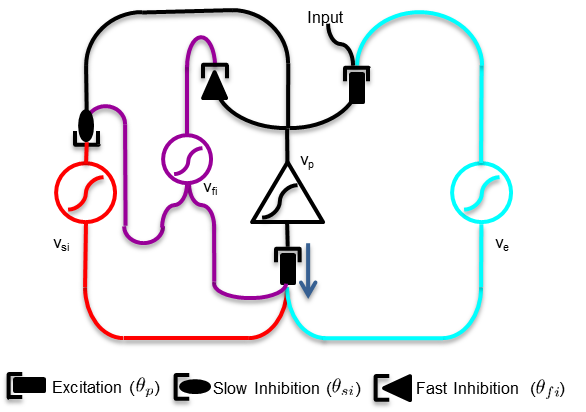
\includegraphics{Biological_Model_DescriptionMin.png}
	\caption{Graphical Description of the Wendling model (Minimised). Membrane potentials are shown and named $v_{b}$ where $b$ is $p$, $e$, $fi$ and $si$ for pyramidal, excitatory and slow and fast inhibitory populations, respectively. The synaptic gains of each population are specified by $\theta_{m}$ where $m$ is defined in the same manner as the membrane potentials and $\theta_{p}=\theta_{e}$. Each triangle and circle indicates a neural population. In particular, the triangle shape indicates the pyramidal population and the circle shapes represent interneurons. The triangles and circles model the action of the soma for the neural populations, and convert membrane potentials to firing rates. The synapses convert the firing rates to membrane potentials. Lastly, each line indicates a neural connection, which is specified by a connectivity constant.}
	\label{fig: BiologicalMin}
\end{figure}%%%%%%%%%%%%%%%%%%%%%%%%%%%%%%%%%%%%%%%%%%%%%

Now consider the full set of original model equations that would be required to specify figure~\ref{fig: Biological}
\begin{align}
\label{eqn: Fullmodel Descrip}
\mathrm{d}v_{po*}(t)&= z_{po*}(t)\mathrm{d}t\\
\mathrm{d}z_{po*}(t)&=\left(\frac{\theta_{p}(t)}{\tau_{p}}c_{1}g(v_{p}(t))-2\frac{z_{po*}(t)}{\tau_{p}}-\frac{v_{po*}(t)}{\tau_{p}^{2}}\right)\mathrm{d}t\\
\mathrm{d}v_{p1*}(t)&= z_{p1*}(t)\mathrm{d}t\\
\mathrm{d}z_{p1*}(t)&=\left(\frac{\theta_{p}(t)}{\tau_{p}}c_{3}g(v_{p}(t))-2\frac{z_{p1*}(t)}{\tau_{p}}-\frac{v_{p1*}(t)}{\tau_{p}^{2}}\right)\mathrm{d}t\\
\mathrm{d}v_{p2*}(t)&= z_{p2*}(t)\mathrm{d}t\\
\label{eqn: Pyr}
\mathrm{d}z_{p2*}(t)&=\left(\frac{\theta_{p}(t)}{\tau_{p}}c_{5}g(v_{p}(t))-2\frac{z_{p2*}(t)}{\tau_{p}}-\frac{v_{p2*}(t)}{\tau_{p}^{2}}\right)\mathrm{d}t\\
\label{eqn: SI}
\mathrm{d}v_{p3*}(t)&= z_{p3*}(t)\mathrm{d}t\\
\mathrm{d}z_{p3*}(t)&=\left(\frac{\theta_{si}(t)}{\tau_{si}}c_{4}g(v_{si}(t))-2\frac{z_{p3*}(t)}{\tau_{si}}-\frac{v_{p3*}(t)}{\tau_{si}^{2}}\right)\mathrm{d}t\\
\mathrm{d}v_{p4*}(t)&= z_{p4*}(t)\mathrm{d}t\\
\label{eqn: SI1}
\mathrm{d}z_{p4*}(t)&=\left(\frac{\theta_{si}(t)}{\tau_{si}}c_{6}g(v_{si}(t))-2\frac{z_{p4*}(t)}{\tau_{si}}-\frac{v_{p4*}(t)}{\tau_{si}^{2}}\right)\mathrm{d}t\\
\label{eqn: FI}
\mathrm{d}v_{p5*}(t)&= z_{p5*}(t)\mathrm{d}t\\
\label{eqn: FI2}
\mathrm{d}z_{p5*}(t)&=\left(\frac{\theta_{fi}(t)}{\tau_{fi}}c_{7}g(v_{fi}(t))-2\frac{z_{p4*}(t)}{\tau_{fi}}-\frac{v_{p5*}(t)}{\tau_{fi}^{2}}\right)\mathrm{d}t\\
\label{eqn: Exc}
\mathrm{d}v_{p6*}(t)&= z_{p6*}(t)\mathrm{d}t\\
\mathrm{d}z_{p6*}(t)&=\left(\frac{\theta_{e}(t)}{\tau_{e}}c_{2}g(v_{e}(t))-2\frac{z_{p6*}(t)}{\tau_{e}}-\frac{v_{p6*}(t)}{\tau_{e}^{2}}\right)\mathrm{d}t\\
\mathrm{d}v_{p7*}(t)&= z_{p7*}(t)\mathrm{d}t\\
\label{eqn: WienerFull}
\mathrm{d}z_{p7*}(t)&=\left(\frac{\theta_{p}(t)}{\tau_{p}}\mu -2\frac{z_{p7*}(t)}{\tau_{e}}-\frac{v_{p7*}(t)}{\tau_{p}^{2}}\right)\mathrm{d}t + \frac{\theta_{p}(t)}{\tau_{p}}\epsilon(t)\mathrm{d}W.\\
\end{align} In these equations $dW$ represents a Wiener process and is required as $\epsilon(t)\sim N(0,\sigma)$, where $\sigma$ and $\mu$ (equation~\ref{eqn: Wiener}) describe the mean and variance of the stochastic model input. Further, $v_{po}(t) $ and $v_{p1-7*}(t)$ represent the membrane potential produced by each synapse and $z_{po*}(t) $ and $z_{p1-7*}(t)$ their derivatives. The inputs to each neural population are specified by $v_{b}(t) $ and $z_{b}(t) $, and are the membrane potential of the specific population, where $b$ takes the values of $p$, $e$, $fi$ and $si$ representing pyramidal, excitatory, and slow and fast inhibitory populations, respectively. Therefore $v_{p}(t) $ is the output of the model. All $v_{b}(t) $ can be described in terms of $v_{po}(t)$ and $v_{p1-7}(t)$ as follows
\begin{align}
\label{eqn: pop1}
v_{p}(t) &= v_{p6*}(t)+v_{p7*}(t)-v_{p3*}(t)-v_{p5*}(t)\\
\label{eqn: pop2}
v_{e}(t) &= v_{po*}(t)\\
\label{eqn: pop3}
v_{si}(t) &= v_{p1*}(t)\\
\label{eqn: pop4}
v_{fi}(t) &= v_{p2*}(t)-v_{p4*}(t).
\end{align} Notice that equations~\ref{eqn: Fullmodel Descrip}-\ref{eqn: Pyr} and equations~\ref{eqn: SI}-\ref{eqn: SI1} are identical except for the connectivity constants. Further, in this model it is assumed that 
\begin{align}
\theta_p = \theta_e\\
\tau_p = \tau_e.
\end{align} Therefore, equations~\ref{eqn: Exc}-\ref{eqn: WienerFull} are identical, but have different inputs. Next consider the effect of the states $v_{p0-7*}(t)$ and $z_{p0-7*}(t)$ on the model inputs. Note that since the effect of $v_{p6*}(t)$ and $v_{p7*}(t)$ are additive, they can be added prior to being passed through the linear filter since
\begin{align}
f{x} + f{y} = f{x+y},
\end{align} where f is defined above and $x$ and $y$ are arbitrary variables. Therefore equations~\ref{eqn: Exc}-\ref{eqn: WienerFull} can be simplified to the following:
\begin{align}
\mathrm{d}v_{p1}(t)&= z_{p1}(t)\mathrm{d}t\\
\label{eqn: Wiener1}
\mathrm{d}z_{p1}(t)&=\left(\frac{\theta_{e}(t)}{\tau_{e}}(\mu +n_{e}g(v_{e}(t))-2\frac{z_{p1}(t)}{\tau_{e}}-\frac{v_{p1}(t)}{\tau_{e}^{2}}\right)\mathrm{d}t + \frac{\theta_{e}(t)}{\tau_{e}}\epsilon(t)\mathrm{d}W.
\end{align}. By making this reduction the effect of both the excitatory population and the input have been incorporated in one potential. Therefore, $v_{p7*}(t)$ is no longer required in equations~\ref{eqn: pop1}. 

Next consider the equations that only have connectivity constants that are different. Notice that these connectivity constants scale the input to the function, and this scaling can be performed after the input is transformed by the linear function. Therefore, equations~\ref{eqn: Fullmodel Descrip}-\ref{eqn: Pyr} can be represented by a single equation such that
\begin{align}
\mathrm{d}v_{po}(t)&= z_{po}(t)\mathrm{d}t\\
\mathrm{d}z_{po}(t)&=\left(\frac{\theta_{p}(t)}{\tau_{p}}g(v_{p}(t))-2\frac{z_{po}(t)}{\tau_{p}}-\frac{v_{po}(t)}{\tau_{p}^{2}}\right)\mathrm{d}t.
\end{align} Notice that in doing this equations~\ref{eqn: pop2}-\ref{eqn: pop4} are no longer valid and need to be altered to include the connectivities that have been removed from their relevant functions
\begin{align}
\label{eqn: pop2n}
v_{e}(t) &= c_{1}v_{po}(t)\\
\label{eqn: pop3n}
v_{si}(t) &= c_{3}v_{p0}(t)\\
\label{eqn: pop4n}
v_{fi}(t) &= c_{5}v_{p0}(t)-v_{p4*}(t).
\end{align}. 

A similar argument can be applied to equations~\ref{eqn: SI}-\ref{eqn: SI1} which can be simplified to
\begin{align}
\mathrm{d}v_{p2}(t)&= z_{p2}(t)\mathrm{d}t\\
\mathrm{d}z_{p2}(t)&=\left(\frac{\theta_{si}(t)}{\tau_{si}}g(v_{si}(t))-2\frac{z_{p2}(t)}{\tau_{si}}-\frac{v_{p2}(t)}{\tau_{si}^{2}}\right)\mathrm{d}t.
\end{align} Again by doing so equation~\ref{eqn: pop1} and~\ref{eqn: pop4n} are no longer valid and become
\begin{align}
v_{p}(t) &= v_{p1}(t)-c_{4}v_{p2}(t)-v_{p5*}(t)\\
v_{fi}(t) &= c_{5}v_{p0}(t)-c_{6}v_{p2}(t).
\end{align}. Lastly for simplicity equations~\ref{eqn: FI}-\ref{eqn: FI2} are replaced with
\begin{align}
\mathrm{d}v_{p3}(t)&= z_{p3}(t)\mathrm{d}t\\
\label{eqn: FI1}
\mathrm{d}z_{p3}(t)&=\left(\frac{\theta_{fi}(t)}{\tau_{fi}}c_{7}g(v_{fi}(t))-2\frac{z_{p3}(t)}{\tau_{fi}}-\frac{v_{p3}(t)}{\tau_{fi}^{2}}\right)\mathrm{d}t.
\end{align} Which results in the set of equations demonstrated in the methods section. Notice that the $n_{b}$ term used in the general form of the equations specifies connectivities that were not removed from the full model description equations due to simplification.



\bibliographystyle{apalike}
\bibliography{RealData}


\end{document}

